\documentclass[11pt,professionalfonts]{beamer}
\usefonttheme{serif}

\usepackage{presentation_packages}
\bibliography{library} % must be in the preamble when using biblatex package

\definecolor{mygray}{gray}{0.9}
\definecolor{RoyalBlue}{rgb}{0.25,0.41,0.88}
\def\Emph{\textcolor{RoyalBlue}}

\definecolor{tmp}{rgb}{0.804,0.941,1.0}
\setbeamercolor{numerical}{fg=black,bg=tmp}
\setbeamercolor{exact}{fg=black,bg=red}

\mode<presentation> 
{
  \usetheme{Warsaw}
  \usefonttheme{serif}
  \setbeamercovered{transparent}
}

\setbeamertemplate{footline}%{split theme}
{%
  \leavevmode%
  \hbox{\begin{beamercolorbox}[wd=.5\paperwidth,ht=2.5ex,dp=1.125ex,leftskip=.3cm,rightskip=.3cm plus1fill]{author in head/foot}%
    \usebeamerfont{author in head/foot}\insertshorttitle
  \end{beamercolorbox}%
  \begin{beamercolorbox}[wd=.5\paperwidth,ht=2.5ex,dp=1.125ex,leftskip=.3cm,rightskip=.3cm]{title in head/foot}
%    \usebeamerfont{title in head/foot}\mypaper\hfill \insertframenumber/\inserttotalframenumber
    \usebeamerfont{title in head/foot}\hfill \insertframenumber/\inserttotalframenumber
  \end{beamercolorbox}}%
  \vskip0pt%
} \setbeamercolor{box}{fg=black,bg=yellow}


\title[Newton's Method]{\large \textbf{Newton's Method}}

\author{\vspace*{-0.3cm}}

   
\institute{
  \footnotesize
  {\normalsize\bf{Shankar Kulumani}}\\
  \vspace*{0.2cm}
    \textbf{Flight Dynamics \& Control Lab}\\ \vspace*{0.5cm}
  \begin{figure} %figure%
        
\includegraphics[width=0.75\textwidth]{figures/gw_txh_2cs_pos.pdf}
    \end{figure}
}
\date{}

\begin{document}
%=======================================================%

\setcounter{framenumber}{-1}
\begin{frame} %-----------------------------%
  \titlepage
\end{frame}   %-----------------------------%

\section*{}
\subsection*{Implicit Equations}  

\begin{frame}{Why?}
\begin{itemize}
    \item Frequently you'll encounter transcendental equations - cannot be solved analytically
    \item However, you can still get a numerical solution using an iterative method
    \item One common problem in astro - solving Kepler's problem
        \begin{equation*}
            \nu_i \to E_i \to M_i \to M_f \to E_f \to \nu_f
        \end{equation*}
\end{itemize}
\end{frame}

\begin{frame}{Iteration}
    \begin{itemize}
        \item Problem occurs in going from \( M_f \) to \( E_f\)
            \begin{align*}
                M_f &\to E_f \\
                M_f &= E_f - e \sin E_f
            \end{align*}
        \item There's no way to directly solve for \( E_f \) given \( M_f, e\)
        \item Instead we'll use Newton's method to find an approximate solution
    \end{itemize}
\end{frame}

\begin{frame}{Newton's Method}
    \begin{itemize}
        \item Find the root, or zero, of a function
        \item Given: \( f(x) \) 
        \item Want: \( x_f \) such that \( f(x_f) = 0 \)
        \item Solution approach:
            \begin{itemize}
                \item Guess a value \( x_0 \) that's close to the true answer
                \item Improve our guess \( x_1 = x_0 - \frac{f(x_0)}{f^{\prime}(x_0)}\)
                \item Repeat until ``close'' enough
                    \begin{align*}
                        x_{n+1} = x_n - \frac{f(x_n)}{f^{\prime}(x_n)}
                    \end{align*}
            \end{itemize}
    \end{itemize}
\end{frame}

\begin{frame}[fragile]{Implement for Kepler's Problem}
    \begin{itemize}
        \item For our problem
            \begin{align*}
                f(E) &= M - (E - e \sin E) \\
                f^{\prime}(E) &= - ( 1 - e \cos E)
            \end{align*}
        \item So for our problem, our iteration method becomes
            \begin{align*}
                E_{n+1} = E_n  + \frac{M - (E - e \sin E)}{1 - e \cos E}
            \end{align*}
        \item What is a good initial guess? - Usually \( M \approx E \) so using \( M_f \) is a good guess
        \item Make sure you use radians or else the answers will be wrong!
        \item When do we stop? - look at the difference in \( E_{n+1} \) and \( E_n \)
\begin{verbatim}
    while np.absolute(Enext - Eprev) < 1e-8:
        loop
    \end{verbatim}
    \end{itemize}
\end{frame}

\begin{frame}{Example - Write a function to solve this!}
    \begin{itemize}
        \item Given: \( M_f = \SI{1.5}{\radian} \) and \( e = 0.1 \)
        \item Find: \( E_f\)
        \item How should we test?
    \end{itemize}
    \begin{figure}
        \centering
        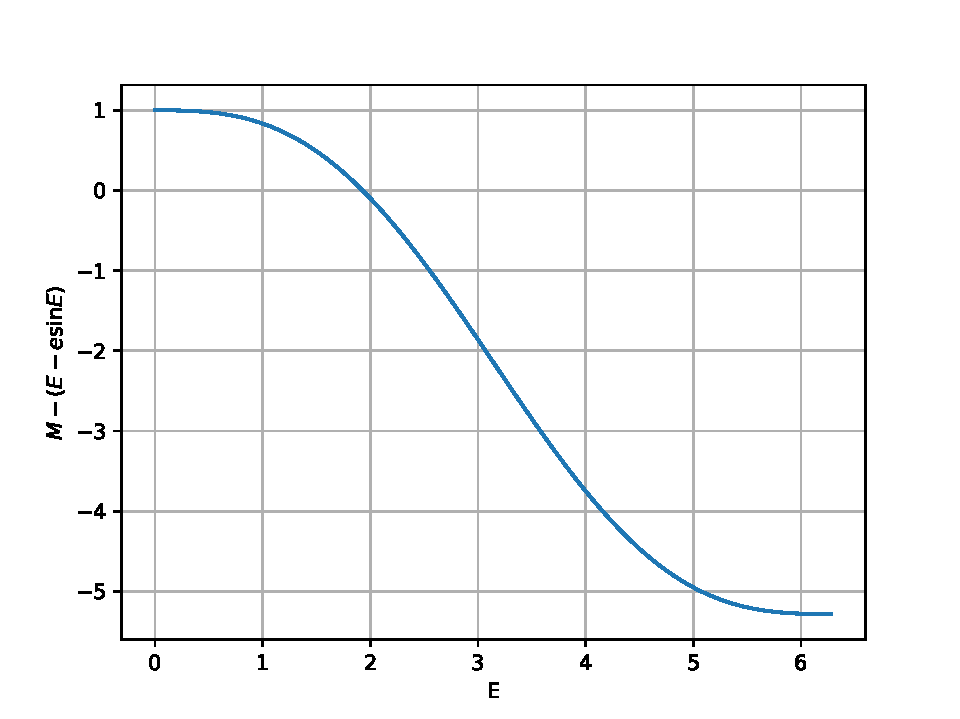
\includegraphics[width=\textwidth,height=0.7\textheight,keepaspectratio]{figures/kepler_eq.pdf}
    \end{figure}
\end{frame}
\end{document}

